\documentclass{jsarticle}
\usepackage[dvipdfmx]{graphicx}
\begin{document}

\title{ライフゲームを作ろう}
\author{宇佐美雅紀}
\maketitle

Haskellの練習として、ライフゲームを作成します。

\section{ライフゲームとは}
ライフゲームは、生命の誕生、進化、淘汰などのプロセスを簡易的なモデルで再現したシミュレーションゲームであり、セル・オートマトンの一種です。
詳しくは、Wikipediaでライフゲームを検索してみてください。
\begin{verbatim}
( http://ja.wikipedia.org/wiki/%E3%83%A9%E3%82%A4%E3%83%95%E3%82%B2%E3%83%BC%E3%83%A0 )
\end{verbatim}

\section{ライフゲームのルール}
\subsection*{誕生}
死んでいるセルに隣接する生きたセルがちょうど3つあれば、次の世代が誕生する。

\subsection*{生存}
生きているセルに隣接する生きたセルが2つか3つ以下ならば、次の世代でも生存する。

\subsection*{過疎}
生きているセルに隣接する生きたセルが1つ以下ならば、過疎により死滅する。

\subsection*{過密}
生きているセルに隣接する生きたセルが4つ以上ならば、過密により死滅する。

\begin{center}
 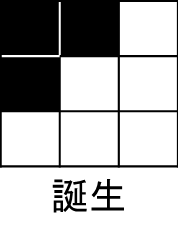
\includegraphics[width=2cm]{reproduction.png}
 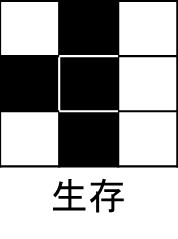
\includegraphics[width=2cm]{next-generation.png}
 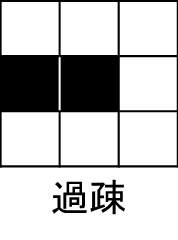
\includegraphics[width=2cm]{under-population.png}
 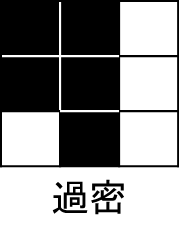
\includegraphics[width=2cm]{overcrowding.png}
\end{center}

\section{ライフゲームのデータ構造}
ライフゲームは任意のサイズ(NxM)の格子状のゲーム盤上で動作します。
ここでは、簡単のために格子のサイズは縦横同じとします(NxN)。
格子の各マスは、生きているか死んでいるかのどちらかです。

レコード構文を使って、以下のように定義します。
\begin{verbatim}
 data Lifegame = Lifegame { size :: Int
                           , life :: [(Int, Int)]
                           }
\end{verbatim}

lifeはタプルのリストで、ゲーム盤上で生きているセルがいる場所を示します。
タプル(ダブル)はゲーム盤上の位置(x座標、y座標)を示します。
タプルが指示していない位置は、生きているセルがいません。

\begin{center}
 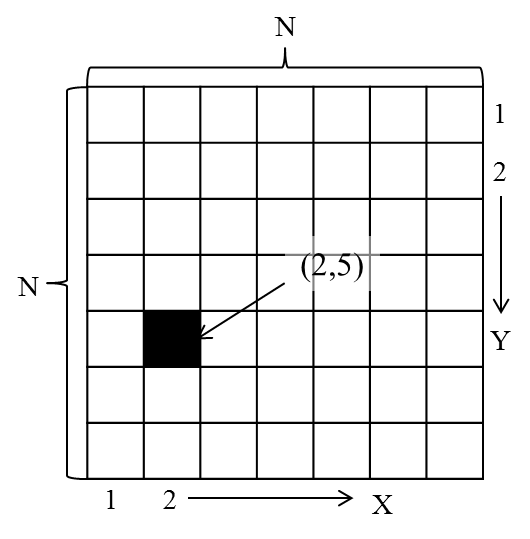
\includegraphics[width=4cm]{gameboard.png}
\end{center}


ここで図が欲しいな~



\end{document}
